\subsection{良好实验在统计上的体现}
我们知道这样一个事实,随机区组设计可以带走区组变量引起的无关变异,重复测量设计可以带走被试个体带来的无关变异,这样实验的结果就更加精确了.
本书的目的是从数据的角度上展示,用了好的实验设计后,更精确的实验的结果的体现.
我们将实验设计与方差分析结合,从数据上看看为什么好的实验设计可以使$F$增大.我们知道:

\[ F = \frac{MSA}{MSE} \]

想让$F$变大有两个手段,让处理效应($MSA$)变大,或者让误差效应($MSE$)变小,这件事情在前面已经介绍过.心理学家感兴趣的那些现象往往都不太明显,人为加大处理效应也没有意义.那么,减小误差才是关键.

\begin{marginfigure}
	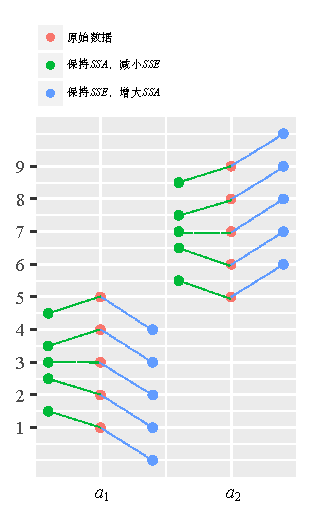
\includegraphics{SSA_SSE}
	\caption{红色是原始数据,蓝色代表组内误差不变,加大处理效应;绿色代表组间变异不变,改变组内误差}
	\labfig{SSA_SSE}
\end{marginfigure}

这就好比用天文望远镜观测外太空,我想发现星星并用我自己的名子命名.我透过天文望远镜看到了一些没有规律发亮的光点,也就是噪音.它们是附近一些已知的行星发出的,也可能是从隔着很远的地方的某个星体传过来的,总之它们像背景一样衬托在我感兴趣的那个星星所发出的光下面.我感兴趣的那颗星星也在发光,不过我现在还不知道这个星星是否真的存在,但我知道,如果这个星星真的存在,它一定会努力发光,并且会和周围那样噪音有显著区别.
事情不是那么容易,星星发的光和噪音总是同时出现,只有星星发出的光足够大,大到和周围的噪音是那么的与众不同,我才敢认定那是星星.我们清楚地知道,想要更加清楚地观察到星星无非有两种手段,其一是让星星在原有基础上多发电光;其二是让周围的噪音降低点.不过好像第一种手段听起来有点滑稽.

方差分析模型中的$MSA$和$MSE$是相互独立的,它们俩可以独立地变化.随机误差指的是由随机因素导致数据在理想值周围随机晃动的偏差,处理效应是人为控制自变量在不同水平上的系统变异,由完全不相干的两个东西导致当然它们是独立的了.下面是一道很重要的思考题:

\begin{kaobox}[frametitle=思考]
假定我们有一组分数,分别计算出$MSA$和$MSE$.\\
(1)我们可以改变$AS$\sidenote[*5][]{$AS$中A代表因素$A$的处理效应,$S$代表被试个体误差,具体是什么后面再说}分数,保持处理平均数恒定.即保持$MSA$不变而改变$MSE$.\\
(2)如果我们改变组平均数,处理组内分数关系不就,$MSA$会变化,而$MSE$不就.表明两个均方是独立变化的.



\end{kaobox}

我们看一组数据
\begin{align*}
    a_1:1, 2, 3, 4, 5\\
    a_2:5, 6, 7, 8, 9
\end{align*}

(1)调整原始数据,保持$SSA$不变,而$SSE$改变(减小$SSE$) (通常加大处理效应实现)

(2)调整原始数据,改变$SSA$不变(增大$SSA$),而$SSE$不变

我直接给出我的思路,\reffig{SSA_SSE}中红色是原始数据,它有两个水平,$a_1$的各个值围绕其均值3波动,$a_2$的各个值围绕其均值7波动.

绿色是我写的符合(1)的一组数据,可以看到红色数据$a_1$处理的每个数据都围绕着3波动,现在绿色的值在$a_1$内还是围绕3波动,但是数据间的距离更短了,它们显得更加紧密.虽然从组内均值上来看(3和7)两组数据的平均值之差不变,但是由于$a_1$的数据更集中于3,$a_2$的数据更集中于7,故实际上这样两组间的差异其实增大了.

蓝色是我写的符合(2)的一组数据,可以看到数据间的紧密程度不变,$a_1$整体向下移动,$a_2$整体向上移动,这样组间的差距被拉大.

原始数据方差分析结果是.

\begin{table}[h]
	\centering
	\caption{原始数据方差分析}
	\labtab{RAW_ANOVA}
	{
		\begin{tabular}{cccccc}
			\toprule
			变异来源 & $SS$ & $df$ & $MS$ & $F$ & $p$  \\
			\midrule
			组间变异 & 40.000 & 1.000 & 40.000 & 16.000 & 0.004  \\
			组内变异 & 20.000 & 8.000 & 2.500 &  &    \\
			\bottomrule
			% \addlinespace[1ex]
			% \multicolumn{6}{p{0.5\linewidth}}{\textit{Note.} Type I Sum of Squares} \\
		\end{tabular}
	}
\end{table}

\begin{margintable}
    \caption{保持$SSA$不变,减小$SSE$}
    \labtab{lower_SSE}
    \raggedright
    \begin{tabular}{cccccc}
        \hline
        $a_1$ & 1.5 & 2.5 & 3 & 3.5 & 4.5\\
        $a_2$ & 5.5 & 6.5 & 7 & 7.5 & 8.5\\
        \hline
    \end{tabular}
\end{margintable}

绿色数据见\vreftab{lower_SSE}.


其方差分析结果是,可以看到相比\vreftab{RAW_ANOVA}中的数据,处理效应没变,误差效应减小了,$F$值变大,$p$值减小.

\begin{table}[h]
	\centering
	\caption{绿色数据方差分析}
	\label{tab:aNOVA-Score}
	{
		\begin{tabular}{cccccc}
			\toprule
			变异来源 & $SS$ & $df$ & $MS$ & $F$ & $p$  \\
			\midrule
			组间变异 & 40.000 & 1.000 & 40.000 & 32.000 & $<$ .001  \\
			组内变异 & 10.000 & 8.000 & 1.250 &  &    \\
			\bottomrule
			% \addlinespace[1ex]
			% \multicolumn{6}{p{0.5\linewidth}}{\textit{Note.} Type III Sum of Squares} \\
		\end{tabular}
	}
\end{table}

\begin{margintable}
    \caption{保持$SSE$不变,增大$SSA$}
    \labtab{UPPER_SSA}
    \raggedright
    \begin{tabular}{cccccc}
        \hline
        $a_1$ & 1 & 1 & 2 & 3 & 4\\
        $a_2$ & 6 & 7 & 8 & 8 & 10\\
        \hline
    \end{tabular}
\end{margintable}

蓝色数据见\vreftab{UPPER_SSA}.

其方差分析结果是,可以看到相比\vreftab{RAW_ANOVA}中的数据,处理效应变大,组内误差减没变,$F$值变大,$p$值减小.

\begin{table}[h]
	\centering
	\caption{蓝色数据方差分析}
	\label{tab:aNOVA-Score}
	{
		\begin{tabular}{cccccc}
			\toprule
			变异来源 & $SS$ & $df$ & $MS$ & $F$ & $p$  \\
			\midrule
			组间变异 & 90.000 & 1.000 & 90.000 & 36.000 & $<$ .001  \\
			组内变异 & 20.000 & 8.000 & 2.500 &  &    \\
			\bottomrule
			% \addlinespace[1ex]
			% \multicolumn{6}{p{0.5\linewidth}}{\textit{Note.} Type III Sum of Squares} \\
		\end{tabular}
	}
\end{table}